%!TEX root = ../main.tex

\chapter{Reti di Hopfield}
\label{cha:reti_di_hopfield}

In questo capitolo considereremo le reti neurali viste come \textbf{sistemi dinamici}\footnote{Un sistema dinamico è un modello matematico utilizzato per descrivere situazioni il cui stato varia nel tempo.} non lineari, con particolare attenzione al problema della loro stabilità o neurodinamica (vedi appendice~\ref{cha:sistemi_dinamici}): per introdurre la variabile tempo in una rete è sufficiente aggiungere dei cicli, ovvero operare con \textbf{reti ricorrenti}.

Le reti ricorrenti con unità non lineari sono generalmente difficili da analizzare: possono convergere a uno stato stabile, oscillare o seguire \textbf{traiettorie caotiche} il cui andamento non è prevedibile.

Tuttavia, il fisico americano J. J. Hopfield si accorse che se le connessioni sono \textbf{simmetriche} esiste una funzione di \textbf{energia globale}. Le reti di Hopfield sono:
\begin{itemize}
	\item \textbf{reti ricorrenti ad uno strato} in cui ogni neurone è connesso a tutti gli altri (escluso sè stesso);
	\item \textbf{simmetriche}: perché hanno la matrice dei pesi sinaptici simmetrica, ovvero $\mat{W}=\mat{W}^T$;
	\item \textbf{non lineari}: nella formulazione continua, ogni neurone ha una funzione di attivazione non lineare invertibile.
\end{itemize}

\begin{figure}[h!]
	\centering
	\begin{tikzpicture}[->,>=stealth',shorten >=1pt,auto,node distance=4cm, semithick]
		\tikzstyle{every state}=[align=center, fill=blue!20,draw=blue]
		
		% Draw nodes.
		\node[state] (1) {$1$};
		\node[state, right of=1] (2) {$2$};
		\node[state, right of=2] (N) {$N$};
        
		% Draw edges
		\path 
		(1) edge[bend left, below] node {$w_{12}$} (2)
		(1) edge[bend left] node {$w_{1N}$} (N)
		(2) edge[bend left] (1)
		(2) edge[bend left] (N)
		(N) edge[bend left] (1)
		(N) edge[bend left] (2)
		(2) edge[dotted, -] (N);
        
	\end{tikzpicture}
	\caption{Una rete ricorrente.}
\end{figure}

\noindent Per quanto riguarda l'aggiornamento di un neurone si possono scegliere tre strade diverse:
\begin{itemize}
	\item \textbf{aggiornamento asincrono}, in cui si aggiorna un neurone alla volta;
	\item \textbf{aggiornamento sincrono}, dove tutti i neuroni vengono aggiornati nello stesso istante;
	\item \textbf{aggiornamento continuo}, in cui tutti i neuroni si aggiornano continuamente.
\end{itemize}
Esistono infine due formulazioni del modello di Hopfield, \textbf{discreto} e \textbf{continuo}, che si differenziano per la modalità di scorrimento del tempo.

\begin{figure}[h!]
	\centering
	\subfigure[Caso discreto: $\Delta t$ costante]{
	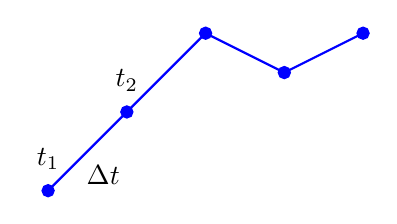
\begin{tikzpicture}
		\draw[thick, color=blue] plot [mark=*,blue, tension=1]
		coordinates{(0, 0) (1, 1) (2, 2) ( 3, 1.5) (4, 2)};
		\node[] at (0, 0.4) {$t_1$};
		\node[] at (0.7, 0.2) {$\Delta t$};
		\node[] at (1, 1.4) {$t_2$};
	\end{tikzpicture}}
	\quad
	\subfigure[Caso continuo: $\Delta t \rightarrow 0$]{
	\begin{tikzpicture}
		\draw[thick, color=blue] plot [smooth, red, tension=1]
		coordinates{(0, 0) (2, 2) ( 3, 1.5) (4, 2)};
	\end{tikzpicture}}
	\caption{Confronto tra caso discreto e continuo.}
\end{figure}

\section{Modello di Hopfield: caso discreto}
\label{sec:modello_di_hopfield_caso_discreto}

In questa sezione si considerano reti di Hopfield in cui il tempo scorre in maniera discreta e i neuroni si aggiornano in modo asincrono.

Per quanto riguarda l'input al neurone si adotta lo stesso modello di McCulloch e Pitts, con l'aggiunta di un fattore di influenza esterno:
\begin{displaymath}
	H_i = \underbrace{\sum_{j \neq i} w_{ij} V_j}_\textrm{modello M\&P} + \underbrace{I_i}_\textrm{input esterno}
\end{displaymath}
La funzione di attivazione (discreta) è la seguente:
\begin{align}
	V_i = \begin{cases}
		+1 & \text{se } H_i > 0 \\
		-1 & \text{se } H_i < 0
	\end{cases}\label{eq:learningrule}
\end{align}
L'aggiornamento dei neuroni è un processo casuale e la selezione dell'unità da aggiornare può essere fatta in due modi:
\begin{enumerate}
	\item ad ogni istante temporale si sceglie a caso l'unità $i$ da aggiornare (utile nelle simulazioni);
	\item ogni unità si aggiorna indipendentemente con probabilità costante ad ogni istante.
\end{enumerate}
A differenza delle reti feedforward, una rete di Hopfield è un sistema dinamico: parte da uno stato iniziale
\begin{align*}
	\vec{V}(0) = (V_1(0), \dots, V_n(0))^T
\end{align*}
ed evolve lungo una traiettoria fino a raggiungere un punto fisso in cui $\vec{V}(t+1) = \vec{V}(t)$ (convergenza).
\begin{figure}[h!]
	\centering
	\begin{tikzpicture}
		\node[point] (0) at (-4, 0) {};
		\node[point] (1) at (-2, 2) {};
		\node[point] (2) at (0, -0.4) {};
		\node[point] (3) at (2, 1) {};
		\node[point] (4) at (4, 0) {};
		\node[point] (5) at (6, -0.5) {};
		\node[point] (6) at (8, 0.5) {};
         
		\foreach \x / \y in {0/1,1/2,2/3,3/4,4/5,5/6}
		\path (\x) edge[->] (\y);
         
		\foreach \x in {0,...,6}
		\node[above=2mm of \x] {\small$\vec{V}(\x)$};
         
	\end{tikzpicture}
	\caption{Traiettoria di una rete di Hopfield nel modello discreto.}
\end{figure}

\noindent Per dimostrare la convergenza, introduciamo la \textbf{funzione di energia} $E$ che governa il sistema
\begin{align}
	E = - \frac{1}{2} \sum_{i=1}^n \sum_{\substack{j=1 \\ j \neq i}}^n w_{ij} V_i V_j - \sum_{i=1}^n I_i V_i\label{eq:energy}
\end{align}
dove il fattore $1/2$ è aggiunto perché i termini identici $w_{ij}x_i x_j$ e $w_{ji} x_j x_i$ sono presenti nella doppia sommatoria.

Il seguente teorema fornisce una condizione sufficiente per la convergenza del sistema.
\begin{thm}[Teorema di Hopfield (caso discreto) - J. J. Hopfield, 1982]
	Se la matrice dei pesi di una rete di Hopfield è simmetrica con $\diag(\mat{W}) = \vec{0}$, allora la funzione di energia \eqref{eq:energy} è una funzione di Lyapunov per il sistema, quindi
\begin{displaymath}
	\Delta E = E(t+1) - E(t) \leq 0
\end{displaymath}
con uguaglianza solo quando il sistema ha raggiunto un punto stazionario.
\end{thm}

\begin{proof}[Dimostrazione.]
	Visto che stiamo utilizzando la modalità di aggiornamento asincrono, supponiamo che il neurone $h$ cambi il proprio stato. La differenza di energia è data da:
	\begin{alignat*}{2}
		\Delta E &=&& - \frac{1}{2} \sum_{i=1}^n \sum_{\substack{j=1 \\ j \neq i}}^n w_{ij} V_i(t + 1) V_j(t + 1) - \sum_{i=1}^n I_i V_i(t + 1) \\
		&&& + \frac{1}{2} \sum_{i=1}^n \sum_{\substack{j=1 \\ j \neq i}}^n w_{ij} V_i(t) V_j(t) + \sum_{i=1}^n I_i V_i(t) \displaybreak[3]\\
		&=&& \underbrace{- \frac{1}{2} \sum_{i=1}^n \sum_{\substack{j=1 \\ j \neq i}}^n w_{ij} (V_i(t + 1) V_j(t + 1) - V_i(t) V_j(t))}_\textbf{$A$} \\
		&&& \underbrace{- \sum_{i=1}^n I_i (V_i(t + 1) - V_i(t))}_\textbf{$B$}
	\end{alignat*}
	Per quanto riguarda il termine $B$ abbiamo:
	\begin{align*}
		B &= - \sum_{i=1}^n I_i \Delta V_i \\
		&= - I_h \Delta V_h
	\end{align*}
	Passiamo ora al primo termine $A$; per prima cosa espandiamo la sommatoria isolando il neurone $h$:
	\begin{align*}
		A =& \underbrace{- \frac{1}{2} \sum_{i \neq h} \sum_{j \neq i} w_{ij} (V_i(t + 1) V_j(t + 1) - V_i(t) V_j(t))}_\textrm{$A_1$} \\
		& \underbrace{- \frac{1}{2} \sum_{j \neq h} w_{hj} (V_h(t + 1) V_j(t + 1) - V_h(t) V_j(t))}_\textrm{$A_2$}
	\end{align*}
	Poiché $V_i(t) = V_i(t + 1)$ per $i \neq h$ si può riscrivere $A_1$ come:
	\begin{align*}
		A_1 &= - \frac{1}{2} \sum_{i \neq h} \sum_{j \neq i} w_{ij} (\underbrace{V_i(t + 1)}_\textrm{$=V_i(t)$} V_j(t + 1) - V_i(t) V_j(t)) \\
		&= - \frac{1}{2} \sum_{i \neq h} \sum_{j \neq i} w_{ij} V_i(t) \underbrace{(V_j(t + 1) - V_j(t))}_\textrm{$=\Delta V_j$} \\
		&= - \frac{1}{2} \sum_{i \neq h} w_{ih} V_i(t) \Delta V_h
	\end{align*}
	Per quanto riguarda $A_2$ il procedimento è lo stesso:
	\begin{align*}
		A_2 &= - \frac{1}{2} \sum_{j \neq h} w_{hj} (V_h(t + 1) V_j(t + 1) - V_h(t) V_j(t)) \\
		&= - \frac{1}{2} \sum_{i \neq h} w_{hi} V_i(t) \Delta V_h
	\end{align*}
	Siccome la matrice dei pesi è simmetrica si ha
	\begin{displaymath}
		A = A_1 + A_2 = - \Delta V_h \sum_{i \neq h} w_{ih} V_i(t)
	\end{displaymath}
	da cui:
	\begin{align*}
		\Delta E &= - \Delta V_h \sum_{i \neq h} w_{ih} V_i(t)  - I_h \Delta V_h \\
		&= - \Delta V_h \underbrace{\left[\sum_{i \neq h} w_{ih} V_i(t) + I_h \right]}_\textrm{input di $h$ al tempo $t + 1$} \\
		&= - \Delta V_h H_h(t + 1)
	\end{align*}
	A questo punto è necessario dimostrare che il prodotto $\Delta V_h H_h(t + 1)$ è sempre non negativo, in modo tale da provare la tesi. Per la regola di apprendimento \eqref{eq:learningrule} si ha
	\begin{enumerate}
		\item $\Delta V_h > 0$ se e solo se $H_h(t + 1) > 0$;
		\item $\Delta V_h < 0$ se e solo se $H_h(t + 1) < 0$;
	\end{enumerate}
	quindi il prodotto è sempre non negativo.
\end{proof}

\section{Regola di Hebb}

Nei computer, se si vuole accedere ad una certa informazione, si utilizza il suo preciso indirizzo di memoria: questo tipo di memoria è definita \textbf{byte-addressable memory}. Nel cervello umano, invece, la memoria è indirizzata in base al contenuto, \textbf{content-addressable memory}: ad esempio pensare alla parola \emph{volpe} potrebbe automaticamente attivare memorie relative ad altri animali simili, alla caccia, oppure al concetto di furbizia.

La \textbf{regola di Hebb} è stata introdotta per descrivere questo meccanismo di accesso alle informazioni e si basa sul principio che, se due neuroni si attivano contemporaneamente, la loro interconnessione deve essere rafforzata. In dettaglio il postulato di Hebb afferma:
\begin{quote}
	\emph{Quando un assone di un neurone A è abbastanza vicino da eccitare un neurone B e questo, in modo ripetitivo e persistente, gli invia un potenziale di azione, inizia un processo di crescita in uno o entrambi i neuroni tale da incrementare l'efficienza di A.}
\end{quote}
La memoria è rappresentata da un insieme di $P$ patterns $\vec{x}^\mu$, con $\mu = 1, \dots, P$: quando viene presentato un nuovo pattern $\vec{x}$, la rete tipicamente risponde producendo il pattern salvato in memoria che più somiglia a $\vec{x}$.

In accordo al postulato di Hebb, sono utilizzati pesi proporzionali alla correlazione nell'attivazione tra un neurone pre e post sinaptico
\begin{displaymath}
	w_{ij} = \frac{1}{N} \sum_{\mu = 1}^p x_i^\mu x_j^\mu
\end{displaymath}
dove $N$ è il numero di unità binarie con output $s_1, \dots, s_N$.

Il meccanismo di \textbf{recall} è il seguente:
\begin{displaymath}
	s_i = \sign\left(\sum_j w_{ij} s_j \right)
\end{displaymath}
Ci sono tuttavia alcuni problemi nell'utilizzo di reti di Hopfield come memorie indirizzate dal contenuto:
\begin{itemize}
	\item il numero massimo di pattern\footnote{I pattern sono memorizzati negli stati di equilibrio della rete.} è $0.15 N$;
	\item talvolta la rete produce degli \textbf{stati spuri}, ovvero stati che non fanno parte dei pattern memorizzati;
	\item il pattern evocato non è necessariamente il più simile a quello di input;
	\item i pattern non sono richiamati tutti con la stessa enfasi.
\end{itemize}

\section{Modello di Hopfield: caso continuo}
\label{sec:modello_di_hopfield_caso_continuo}

In questo modello i neuroni non sono più dispositivi binari con stati $(0, 1)$ o $(-1, 1)$, ma producono un output che identifica la quantità di corrente elettrica: lo scopo di Hopfield, infatti, era quello di fornire un'implementazione fisica del suo modello che imiti il più possibile il funzionamento di un cervello biologico.

L'output di un neurone $i$ è dato da
\begin{displaymath}
	V_i = g_\beta(\mu_i) = g_\beta \left(\sum_{j} w_{ij} V_j + I_i \right) 
\end{displaymath}
dove $g_\beta$ è la funzione di attivazione \textbf{crescente}, \textbf{continua} e \textbf{non lineare}. Le funzioni più utilizzate come $g_\beta$ sono la tangente iperbolica e la sigmoidea:
\begin{align*}
	\tanh_\beta(\mu) &= \frac {e^{\beta\mu} - e^{-\beta\mu}} {e^{\beta\mu} + e^{-\beta\mu}} \quad \in\; ]-1,1[ &
	g_\beta(\mu) &=\frac{1}{1 + e^{- \beta \mu}} \quad\in\; ]0,1[
\end{align*}
Il parametro $\beta$ indica la \emph{stickiness} della funzione: per $\beta \rightarrow \infty$ la funzione diventa sempre più ripida fino a diventare una funzione a gradino.

\begin{figure}[h!]
	\centering
	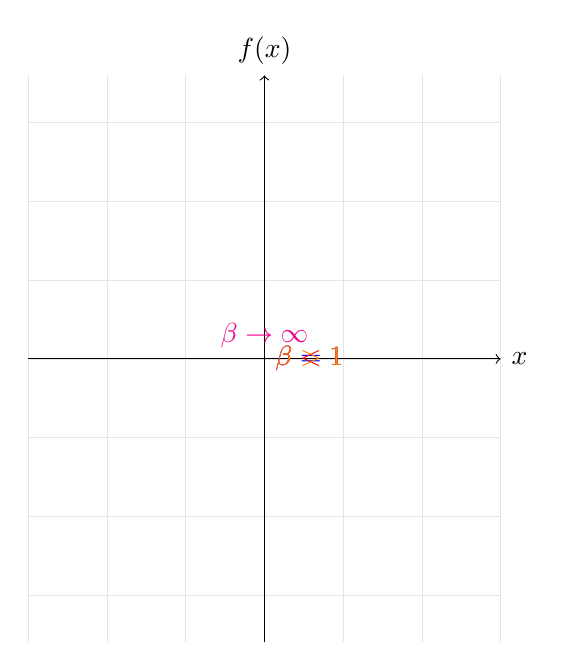
\begin{tikzpicture}[domain=-1:1,x=3cm,y=3cm,  every node/.style=very thick]
		\draw[very thin,color=gray!20] (-1,-1.2) grid (1,1.2);
		\draw[->] (-1,0) -- (1,0) node[right] {$x$};
		\draw[->] (0,-1.2) -- (0,1.2) node[above] {$f(x)$};
		\draw[color=blue] plot[id=tanh] function{tanh(1 * x)} node[right] {$\beta = 1$};
		\draw[color=red] plot[id=tanh] function{tanh(0.5 * x)} node[right] {$\beta < 1$};
		\draw[color=orange] plot[id=tanh] function{tanh(1.5 * x)} node[right] {$\beta > 1$};
		\draw[color=magenta] plot[id=tanh] function{tanh(100 * x)} node[above] {$\beta \rightarrow \infty$};
	\end{tikzpicture}
	\caption{La funzione tangente iperbolica.}\label{fig:stickiness}
\end{figure}

\noindent L'utilizzo di valori continui permette la modalità di \textbf{aggiornamento continuo} dei neuroni. Secondo questa modalità, il sistema evolve in accordo al seguente insieme di equazioni differenziali
\begin{displaymath}
	V_i + \tau_i \frac{\dif V_i}{\dif t} = g_\beta \left(\sum_{j} w_{ij} V_j + I_i \right)
\end{displaymath}
dove $\tau_i$ è una costante positiva che rappresenta la resistenza elettrica. Il sistema raggiunge la stabilità quando $\dif V_i / \dif t= 0 \, \forall i$.

In maniera del tutto equivalente, è possibile esprimere l'equazione di stato non incentrando l'attenzione sulla variazione dello stato $V_i$ nel tempo, quanto sulla variazione dell'input netto $\mu_i$ nel tempo, pervenendo alla seguente equazione:
\begin{displaymath}
	\mu_i + \tau_i \frac{\dif\mu_i}{\dif t} = \sum_j w_{ij} V_j + I_i = \sum_j w_{ij} g_\beta (\mu_j) + I_i \\
\end{displaymath}
La \textbf{funzione energia} nel modello continuo è simile a quella nel caso discreto:
\begin{align}
	E = - \frac{1}{2} \sum_i \sum_j w_{ij} V_i V_j + \sum_i \int_0^{V_i} g^{-1}_\beta (V) \, \dif V - \sum_i I_i V_i \label{eq:energycont}
\end{align}

Analogamente al caso discreto, il seguente teorema fornisce una condizione sufficiente per la convergenza del sistema.
\begin{thm}[Teorema di Hopfield (caso continuo) - J. J. Hopfield, 1982]
	Se la matrice dei pesi di una rete di Hopfield è simmetrica con $\diag(W) = \vec{0}$, allora la funzione di energia \eqref{eq:energycont} è una funzione di Lyapunov per il sistema, quindi $\dif E / \dif t \leq 0$ con uguaglianza quando il sistema ha raggiunto un punto stazionario.
\end{thm}

\begin{proof}[Dimostrazione.]
	Calcoliamo la derivata della funzione energia:
	\begin{align*}
		\frac{\dif E}{\dif t} &= - \frac{1}{2} \sum_i \sum_j w_{ij} \frac{\dif V_i}{\dif t} V_j - \frac{1}{2} \sum_i \sum_j w_{ij} V_i \frac{\dif V_j}{\dif t} + \sum_i \underbrace{g_\beta^{-1}(V_i)}_\textrm{$= \mu_i$} \frac{\dif V_i}{\dif t} - \sum_i I_i \frac{\dif V_i}{\dif t} \\
		\intertext{Per simmetria di $W$ si possono sommare i primi due termini:}
		&=  - \sum_i \sum_j w_{ij} \frac{\dif V_i}{\dif t} V_j + \sum_i \mu_i \frac{\dif V_i}{\dif t} - \sum_i I_i \frac{\dif V_i}{\dif t} \\
		&= - \sum_i \frac{\dif V_i}{\dif t} \underbrace{\left(\sum_j w_{ij} V_j - \mu_i + I_i \right)}_\textrm{$ = \tau_i \frac{\dif \mu_i}{\dif t}$} \\
		&= - \sum_i \tau_i \frac{\dif V_i}{\dif t} \frac{\dif \mu_i}{\dif t} \\
		&= - \sum_i \tau_i g'_\beta(\mu_i) \left(\frac{\dif \mu_i}{\dif t} \right)^2 \leq 0
	\end{align*}
	L'ultima disuguaglianza è verificata poiché $g_\beta$ è crescente, quindi $g'_\beta > 0$, $\tau_i > 0$ per ipotesi e il quadrato di un numero è sempre non negativo. Vale quindi la doppia implicazione
	\begin{align*}
		\frac{\dif E}{\dif t} = 0 \Leftrightarrow \frac{\dif \mu_i}{\dif t} = 0 \,\forall i
	\end{align*}
	cioè il valore dell'energia nel tempo rimane fisso se e solo se la rete ha raggiunto un punto di equilibrio.
\end{proof}

\section{Corrispondenza tra i due modelli}
\label{sec:corrispondenza_tra_i_due_modelli}

Esiste una relazione stretta tra il modello continuo e quello discreto. Si noti che
\begin{align*}
	V_i = g_\beta(\mu_i) = g_1(\beta \mu_i)
\end{align*}
da cui si ricava:
\begin{align*}
	\mu_i = \frac{1}{\beta} g_1^{-1} (V_i)
\end{align*}
Il secondo termine della funzione energia diventa
\begin{align*}
	\sum_i \int_0^{V_i} g_\beta^{-1}(V) \, \dif V = \frac{1}{\beta} \sum_i \int_0^{V_i} g_1^{-1}(V) \, \dif V 
\end{align*}
che, per $\beta \rightarrow \infty$, diventa trascurabile e la funzione di energia risulta uguale a quella nel modello discreto.
\begin{align*}
	E &= - \frac{1}{2} \sum_i \sum_j w_{ij} V_i V_j + \underbrace{\frac{1}{\beta}  \sum_i \int_0^{V_i} g_1^{-1} (V) \, \dif V}_\textrm{= 0 per $\beta \rightarrow \infty$}  - \sum_i I_i V_i \\
	&=  - \frac{1}{2} \sum_i \sum_j w_{ij} V_i V_j - \sum_{i=1}^n I_i V_i
\end{align*}
